\chapter{Constrains using HAWC on GRB170817A}

Desafortunadamente, el evento de la onda gravitacional GW170817 ocurri� fuera del campo de visi�n de HAWC. Sin embargo, 8 hrs depu�s el tr�nsito logra entrar en el campo de visi�n del observatorio colocando un upper limit a XX \citep{2017ApJ...848L..12A} despu�s de $\sim$ 8 hrs. despu�s de la detecci�n por Fermi-GBM. Debido a la naturaleza que present� el afterglow de este GRB, en donde, apareci� la emisi�n de rayos X a 9 d�as \citep{2017Natur.551...71T} y de radio a 16 d�as \citep{2017Sci...358.1579H} despu�s del destello respectivamente, alcanzando un flujo m�ximo a los \textcolor{red}{120 d�as} \citep{2018A&A...613L...1D, 2018ApJ...856L..18M} se realiza un monitoreo a ciegas buscando  emisi�n en TeV's detectable por HAWC.

\begin{figure}[ht!]
  \centering{
  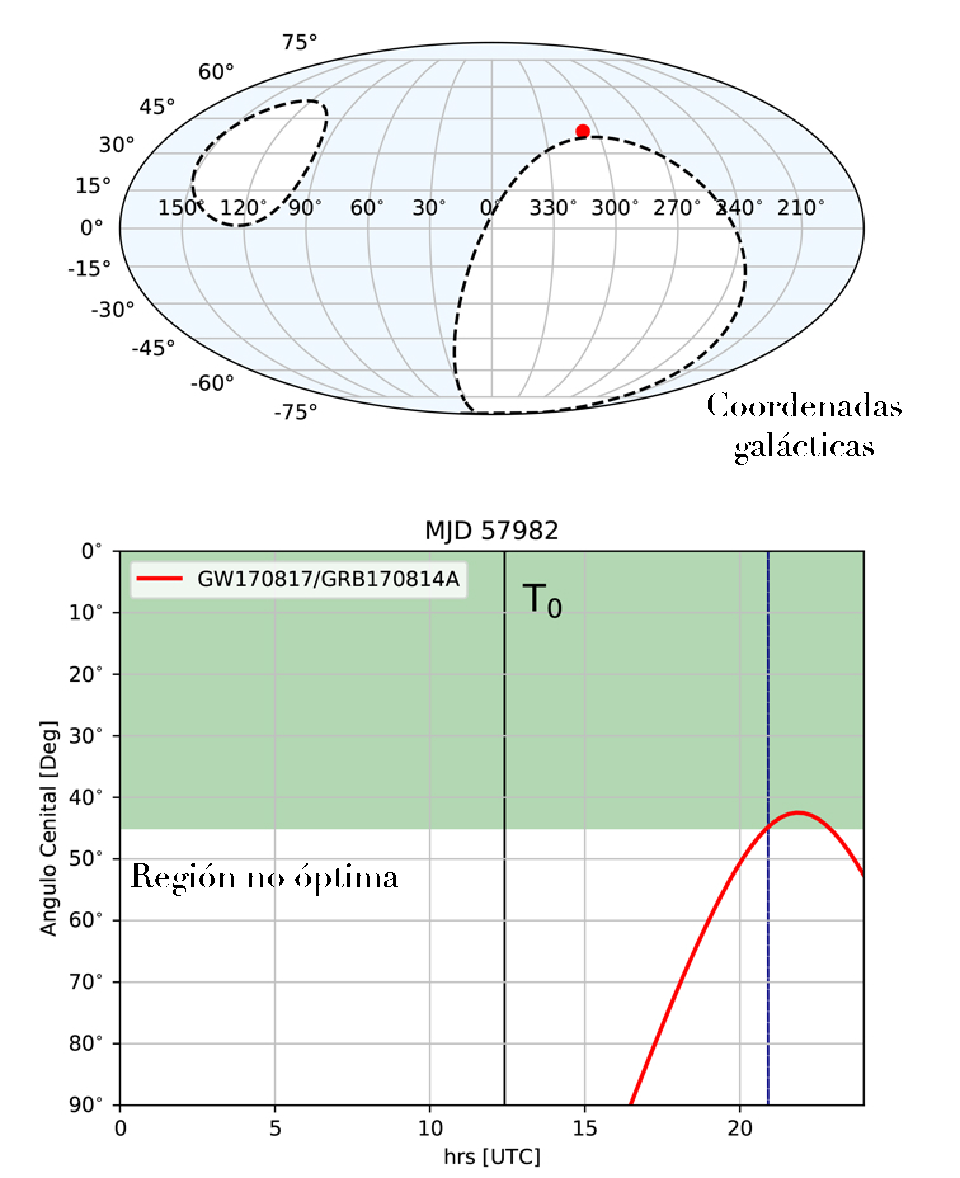
\includegraphics[width=1.0\linewidth]{Figures/HAWC-FOV-Transit.pdf}}
  \caption{Transito de la onda gravitacional sobre HAWC.}
  \label{fig:FOV-HAWC-GW}
\end{figure}


\section{Mapas del cielo de d�as siderales}

HAWC presenta su �ptima sensibilidad para fuentes que se encuentran dentro de las declinaciones -26$\degree$ y +64$\degree$, tal y como se muestra la regi�n sombreada en la figura \ref{fig:FOV-HAWC-GW}. De esta manera definimos a un transito como la visibilidad de una fuente por HAWC la cual se encuentra con un �ngulo cenital $\theta$ < 45$\degree$. Un estudio m�s detallado presentado en \citep{2017ApJ...841..100A} muestra que la mayor cantidad de emisi�n de fuentes c�mo lo son la nebulosa del Cangrejo, y los Markarian 421 y 501 deber�an de detectarse dentro de las primeras 4 hrs del transito sobre HAWC. As� mismo los mapas inician a la media noche sideral de HAWC. Los mapas son dividos en mapas de 12 horas siderias, de tal forma que se genera una subclaficiaci�n, aquellas fuentes las cuales tienen una ascensi�n recta < 3 hrs �  > 21 hrs � bien, el complemento.\\

Cada mapa sideral est� dividido en 9 bines en funci�n de la multiplicidad del primario \citep{2017ApJ...843...39A} y cada bin est� constituido por un mapa utilizando una malla de pixeles mediante HEALPix \citep{2005ApJ...622..759G} considerando una resoluci�n de 1024 pixeles a lo largo de la esfera (cada pixel tiene una separaci�n de 0.06$^{\circ}$). Estos mapas son ampliamente dominados por eventos hadr�nicos, por lo que la estimaci�n del background se obtiene mediante un procedimiento de integraci�n directa \citep{2003ApJ...595..803A, 2017ApJ...843...39A}. Una vez \textcolor{red}{continuar escribiendo ac�}.\\

\section{B�squeda tard�a en TeVs}
Para este trabajo se consideran 3 bines temporales equidistantes logaritmicamente. De tal manera, que el bin $\mathds{B}_{i}$ con i=\{1,2,3\} contiene 1, 10 y 100 d�as respectivamente. Estos intervalos de tiempo son corregidos mediante un corte de calidad, mediante los cuales se busca mitigar periodos de inestabilidad del experimento, de tal forma que podemos asegurar que al menos el 50\% del tr�nsito est� contenido dentro del mapa. La tabla \textbf{[??]} muestra la cantidad de tiempo integrado para los 3 bines.

\begin{table}[]
\centering
\begin{tabular}{ccc}
$\mathds{B}$ & Tiempo total sobre HAWC & Tiempo corregido \\
\hline
\hline
1 & 0 & 0 \\
2 & 0 & 0\\
3 & 0 & 0 
\end{tabular}
\end{table}

\section{L�mites al flujo propuestos y restricci�n a modelos}

Desafortunadamente, este evento no logr� ser detectado por HAWC. As� que son calculados limites superiores en el flujo \citep{1998PhRvD..57.3873F,2017ApJ...843...39A,2017ApJ...843...40A} \textcolor{red}{Continuar escribiendo ac�}.

\begin{figure}[ht!]
  \centering{
  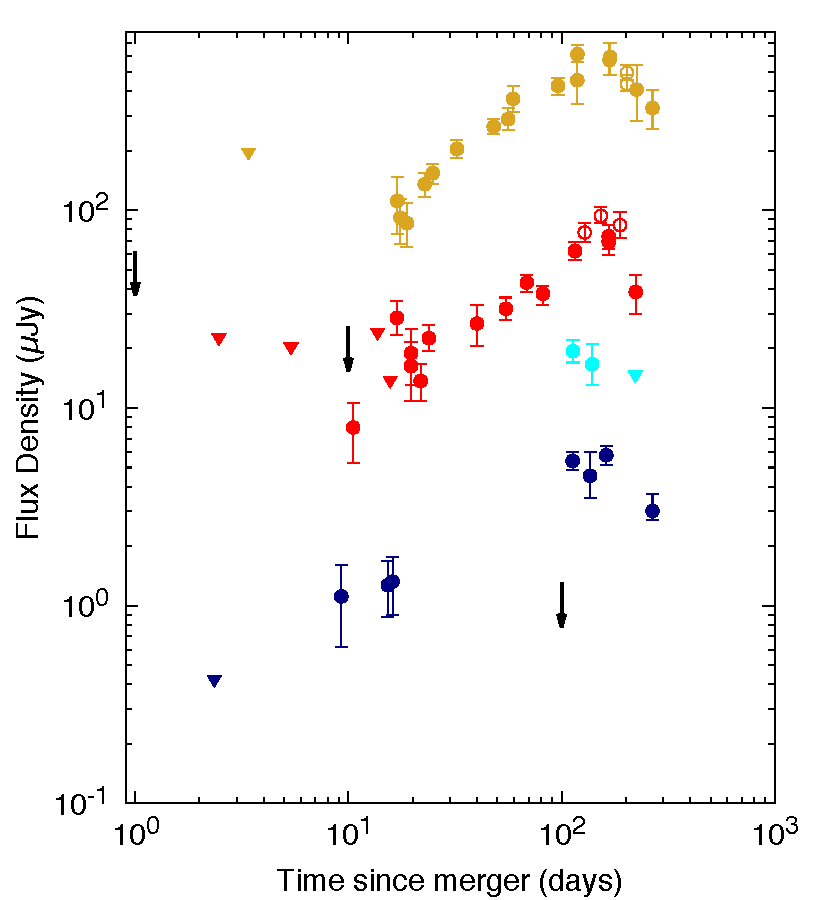
\includegraphics[width=1.0\linewidth]{Figures/LightCurve_GRB170817A.pdf}}
  \caption{Transito de la onda gravitacional sobre HAWC.}
  \label{fig:LC170817A}
\end{figure}